
%%%%%%%%% MASTER -- compiles the 4 sections

%\documentclass[12pt,letterpaper]{article}
\documentclass[12pt,letterpaper,headings=normal]{scrartcl}

%%%%%%%%%%%%%%%%%%%%%%%%%%%%%%%%%%%%%%%%%%%%%%%%%%%%%%%%%%%%%%%%%%%%%%%%%
\pagestyle{plain}                                                      %%
%%%%%%%%%% EXACT 1in MARGINS %%%%%%%                                   %%
\setlength{\textwidth}{6.5in}     %%                                   %%
\setlength{\oddsidemargin}{0in}   %% (It is recommended that you       %%
\setlength{\evensidemargin}{0in}  %%  not change these parameters,     %%
\setlength{\textheight}{8.5in}    %%  at the risk of having your       %%
\setlength{\topmargin}{-.3in}       %%  proposal dismissed on the basis  %%
\setlength{\headheight}{0in}      %%  of incorrect formatting!!!)      %%
\setlength{\headsep}{0in}         %%                                   %%
\setlength{\footskip}{.2in}       %%                                   %%
%%%%%%%%%%%%%%%%%%%%%%%%%%%%%%%%%%%%                                   %%
\newcommand{\required}[1]{\section*{\hfil #1\hfil}}                    %%
\renewcommand{\refname}{\hfil References Cited\hfil}                   %%
\bibliographystyle{plain}                                              %%
%%%%%%%%%%%%%%%%%%%%%%%%%%%%%%%%%%%%%%%%%%%%%%%%%%%%%%%%%%%%%%%%%%%%%%%%%

%\setlength{\textheight}{9.4in}
%\renewcommand{\topfraction}{1}		% max fraction of floats at top
%\renewcommand{\bottomfraction}{1}	% max fraction of floats at bottom
%\def\overheader{-0.1in}
%\def\underheader{-0.1in}

\renewcommand{\rmdefault}{ptm} % Palatino=ppl or Times=ptm
\renewcommand{\sfdefault}{phv} % Helvetica
\renewcommand{\ttdefault}{pcr}  % Courier

\renewcommand{\thesection}{\Alph{section}} % change section nunbering to alphabetic

%PUT YOUR MACROS HERE
\usepackage{comment}
\usepackage{subfigure}
\usepackage{graphicx}
\usepackage{wrapfig}
\usepackage{url}
\usepackage{multicol}
\usepackage[margin=0pt,font=small,labelfont=bf,format=plain]{caption}
\usepackage{fancyhdr}
\usepackage{datetime}
\pagestyle{fancy}
\fancyhf{}
\renewcommand{\headrulewidth}{0pt}
\fancyhead[R]{\vspace{-1.5cm} \textit{Page =}~\thepage}
\usepackage{pdfpages}
\includepdfset{pagecommand=\thispagestyle{fancy}}
\usepackage{epsfig}


\begin{document}

%\markboth{\Large \bf Revised handout}{ }

%\baselineskip=24pt  % Enforce double space

\baselineskip=48pt  % Enforce double space

%\baselineskip=18pt  % Enforce 1.5 space
%
%\setlength{\parskip}{.3in}
%\setlength{\itemsep}{.3in}

\pagestyle{plain}

\vspace*{7cm}


\begin{center}
{\Large
 Rob 501 Handouts \\
 Background Material on Logic and Proofs \mbox{ } \\
\mbox{ } \\
J.W. Grizzle \\
\mbox{ } \\
\mbox{ }
}
%{\bf Compiled on~\today~~at~\currenttime}
\end{center}

\newpage

\newpage
\vspace*{10cm}
{\Large 
\begin{center}
 Introduction to Mathematical Arguments
\end{center}
}
\newpage

\textbf{Sources:}
{\footnotesize
\begin{itemize}
\item Various Proof Techniques\\
\url{http://math.kennesaw.edu/~plaval/math4381/induction.pdf}
\item  Factorization into primes using the Second Principle of Induction [aka Strong Induction].\\ \url{http://courses.engr.illinois.edu/cs173/sp2009/lectures/lect_18.pdf}
\item How to negate statements with quantifiers \\
\url{http://www.math.binghamton.edu/dennis/478.f07/EleAna.pdf}
\end{itemize}
}
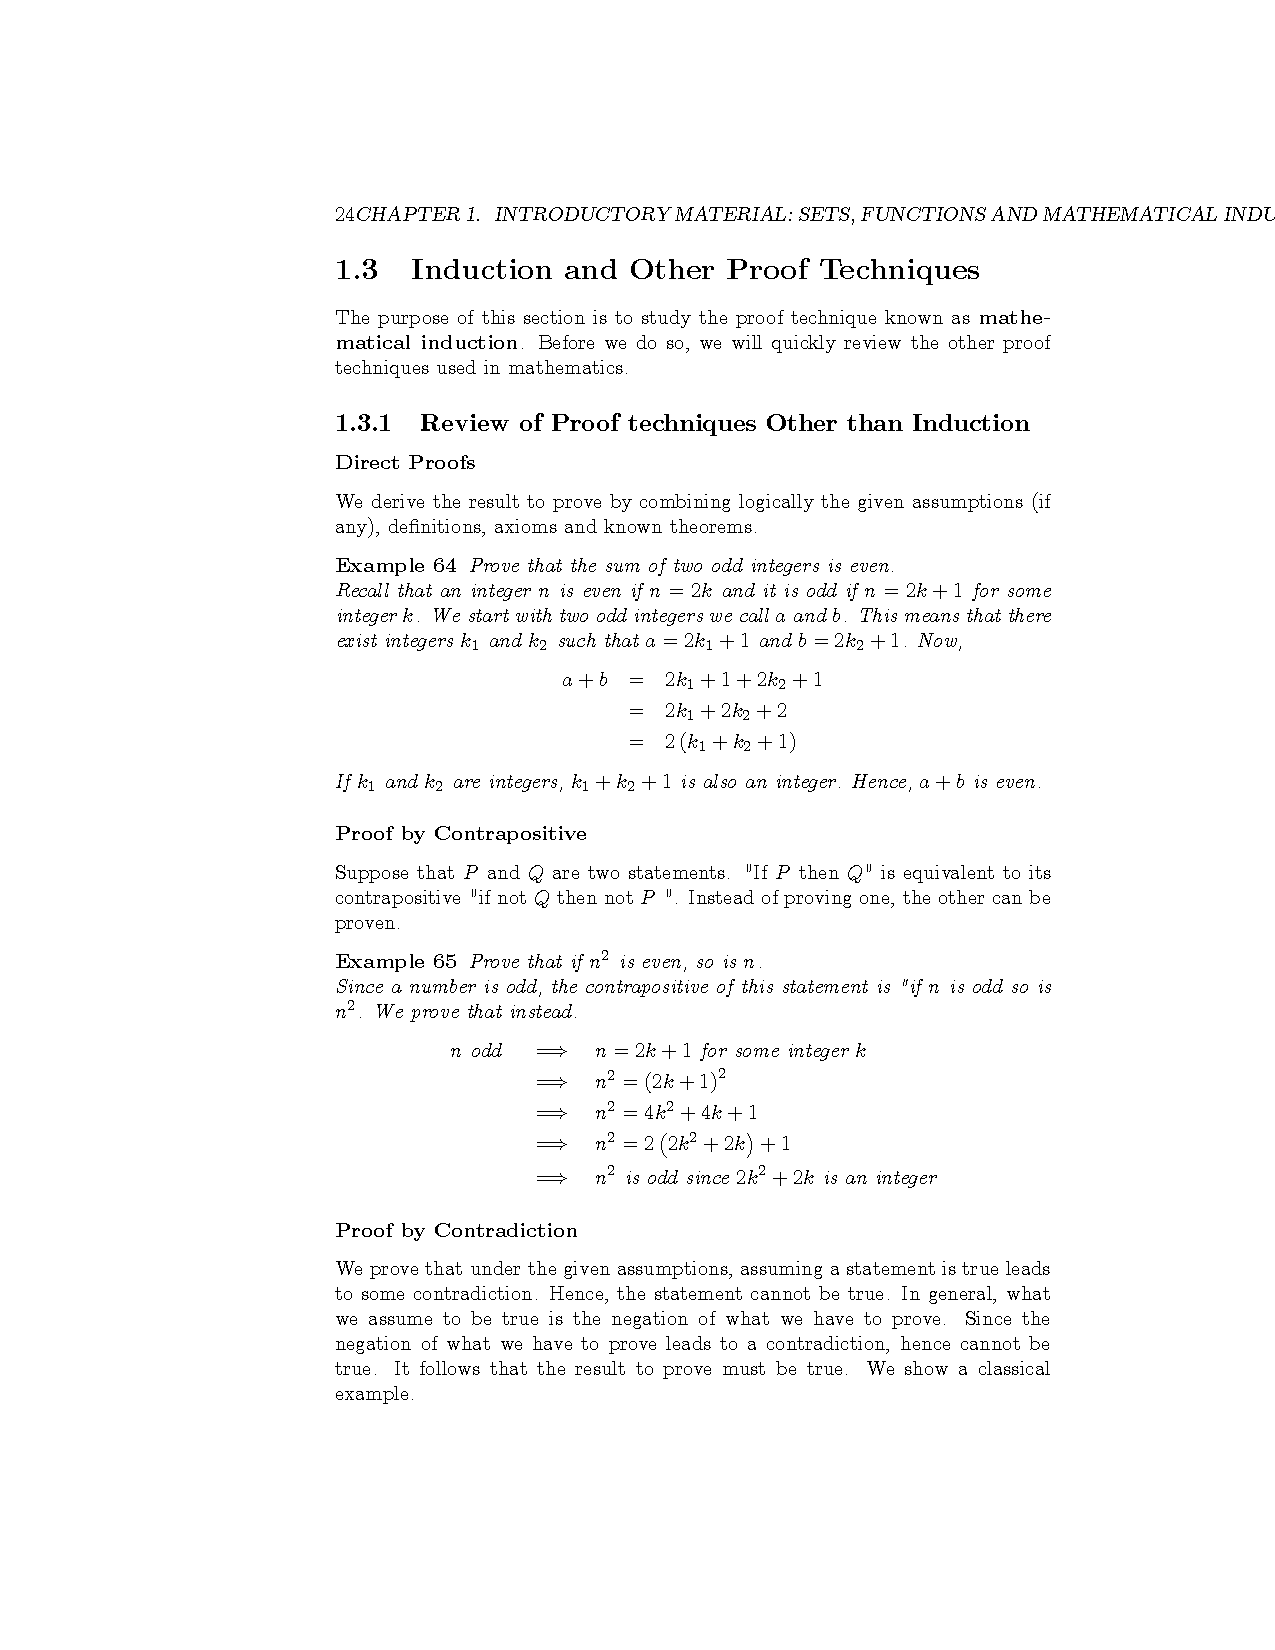
\includepdf[pages=-]{NotesFromWeb/Proofs/Proofs_Direct_Contradiction_Induction.pdf}
\vspace*{\fill}
Factoring Primes Using Strong Induction, Plus Other Examples
\vspace*{\fill}
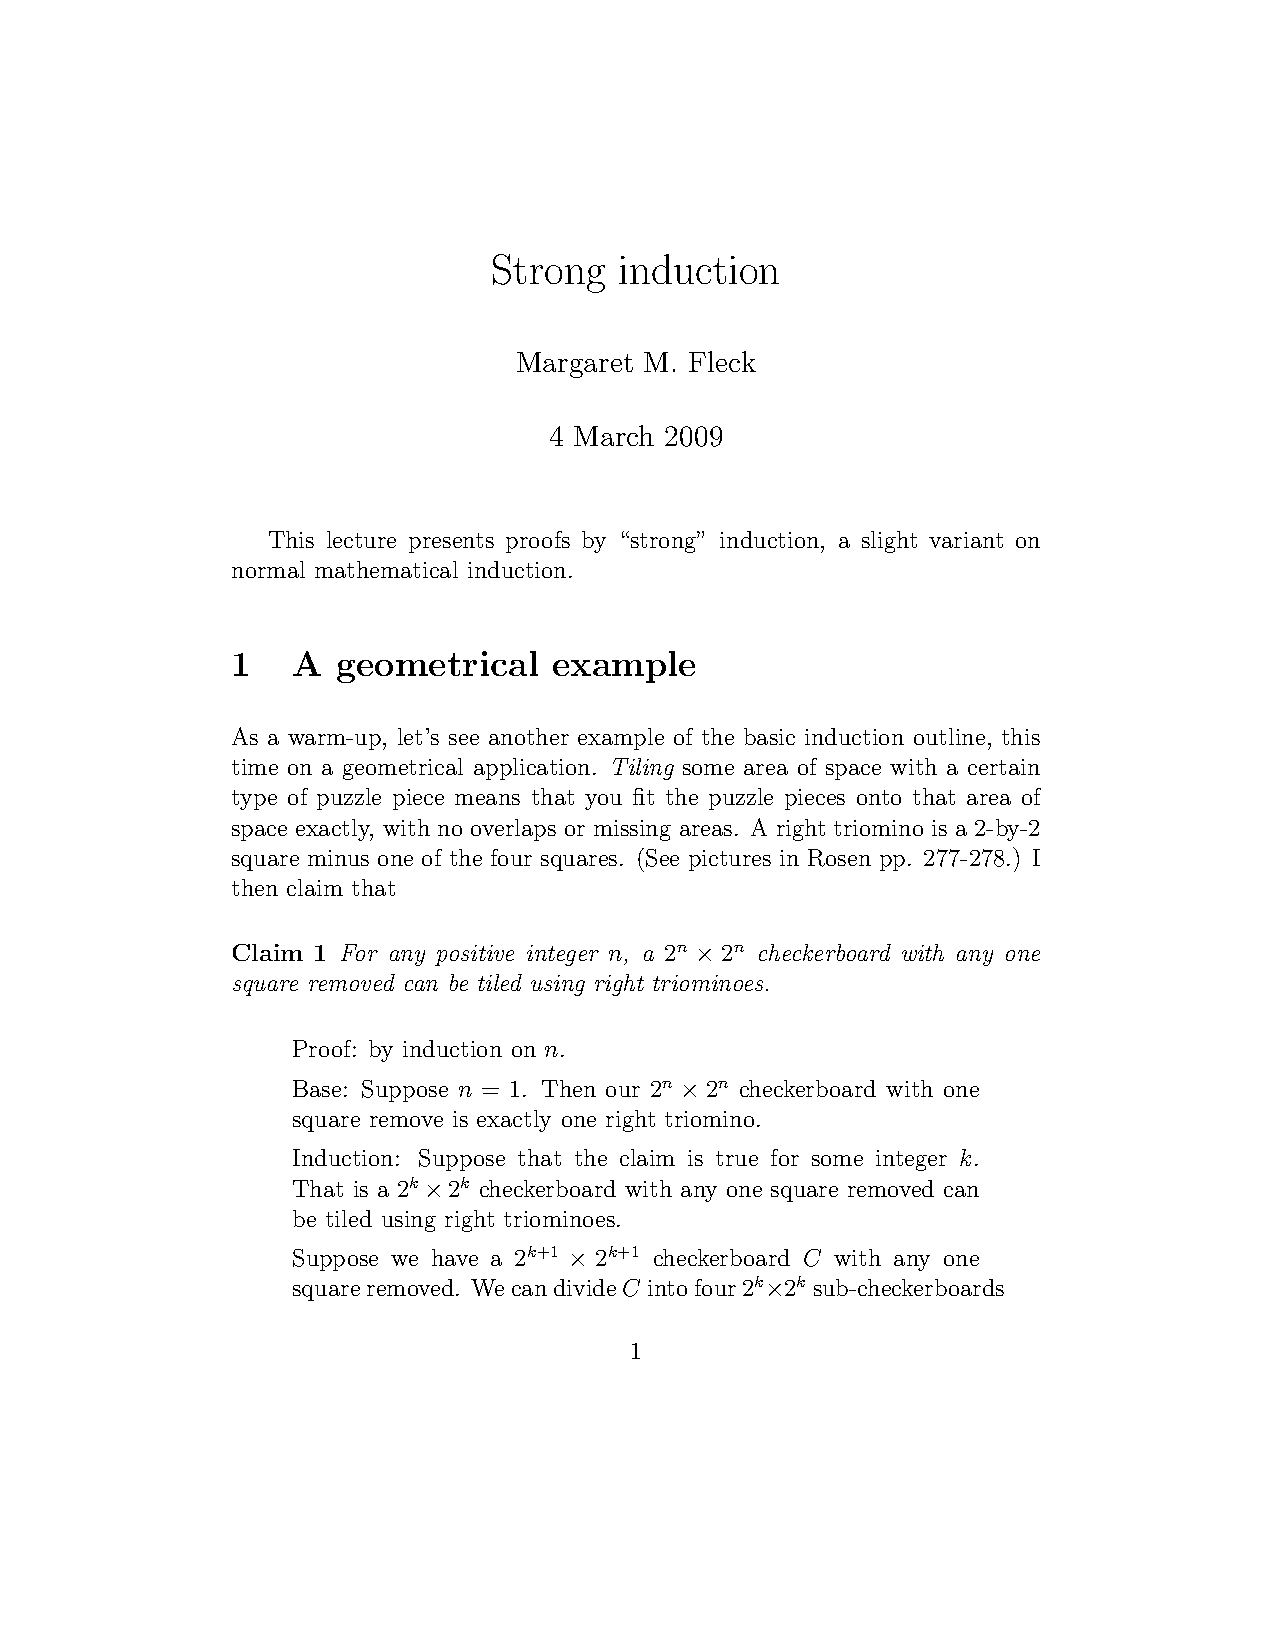
\includepdf[pages=-]{NotesFromWeb/Proofs/Proofs_StrongInduction_lect_18.pdf}
\vspace*{\fill}
How to Negate Statements
\vspace*{\fill}
\includepdf[pages=2-3]{BookChapters/RealAnalysis/Proofs_NegationOfLogicalStatementsFrom_EleAna.pdf}



\end{document}
